% HA-Expert: A Domain-Adapted Language Model and Evidence-Checked
% Benchmark for Hyaluronan Research
% arXiv preprint manuscript (cs.CL primary; cross-list cs.LG, q-bio.BM).
% Sources: notes/arxiv-draft-v1.md; eval/results/s6-full-report.md;
% eval/verify_summary_v3.md; notes/PROJECT_PLAN.md; model card
% (hf-staging/model-card-sft.md). All reported numbers are taken from
% those records.
% Pre-submission notes: (1) an arXiv endorsement code is still required
% before submission; (2) the reference list is the draft's selected list
% and may be completed at submission time.
\documentclass[11pt]{article}

\usepackage[letterpaper,margin=1in]{geometry}
\usepackage{booktabs}
\usepackage{array}
\usepackage{graphicx}
\usepackage{amsmath}
\usepackage{url}
\usepackage{hyperref}
\hypersetup{colorlinks=true, linkcolor=blue, citecolor=blue, urlcolor=blue}

\title{HA-Expert: A Domain-Adapted Language Model and Evidence-Checked
Benchmark for Hyaluronan Research}

\author{Kunli Liu\\
Independent Researcher, San Francisco Bay Area, USA\\
\href{mailto:liukunli001@gmail.com}{liukunli001@gmail.com}}

\date{}

\begin{document}
\maketitle

\begin{abstract}
Specialized scientific fields accumulate knowledge in large, dispersed
literatures that general-purpose language models handle unreliably: answers
are fluent but often wrong on quantitative details, and confident even when
a question's premise is false. We study one such field --- hyaluronan
(hyaluronic acid, HA), a glycosaminoglycan whose research spans
glycochemistry, biomaterials, drug delivery, and clinical medicine --- and
ask how far a single researcher with a modest compute budget can go in
building a \emph{trustworthy} domain model. We release (i) a cleaned
corpus
of 12,306 full-text HA papers ($\sim$126M tokens); (ii) HA-Expert, a
Qwen3-8B-Base model adapted in two stages --- domain-adaptive continued
pretraining (DAPT) on 60M tokens of the corpus, then full-parameter
supervised fine-tuning (SFT) on 12,003 question--answer pairs generated by
the DAPT model itself, at zero API cost --- and optionally grounded at
inference by retrieval over a 636,959-passage FAISS index of the same
corpus; and (iii) HA-Expert-Bench, 240 questions whose reference answers
were verified against retrieved source passages by evidence-restricted LLM
verifiers (212 of 240 confirmed or corrected), including 15
adversarial ``trap'' questions with false premises. In a four-cell
ablation, SFT doubles the base model (0.300 $\rightarrow$ 0.601);
retrieval is the largest single lever (base+RAG 0.710; traps
0.267 $\rightarrow$ 0.867); and SFT and RAG do \textbf{not}
compose additively (0.662): a model that never saw retrieved context in
training collapses into citation-marker loops (5 of 240
retrieval-augmented responses) and inherits its teacher's repetition
habit through self-distillation. Total cloud compute was under USD 50.
All code, data, weights, and the benchmark are publicly released.
\end{abstract}

\section{Introduction}
\label{sec:intro}

Hyaluronan is a linear glycosaminoglycan of repeating
$\beta$-1,4-glucuronic-acid / $\beta$-1,3-$N$-acetylglucosamine
disaccharides, central to extracellular-matrix biology, joint lubrication,
wound healing, ophthalmic and dermal formulations, and drug delivery.
The knowledge a practitioner needs ---
molecular-weight-dependent biology, receptor interactions (CD44, RHAMM,
LYVE-1), chemical modification routes, production methods, clinical
dosing --- is spread across thousands of papers in chemistry, materials,
and medical journals. No textbook tracks it, and the literature grows
faster than anyone can read.

General-purpose LLMs are an attractive interface to such a literature,
but in our initial probes their failures were systematic, and of three
kinds. First, \emph{behavior}: the base model frequently
continued the prompt with invented follow-up questions instead of
answering. Second, \emph{epistemic stance}: it assented to false premises
--- for example, that HA is a protein polymer, or that HA solutions are
Newtonian fluids --- rather than correcting them. Third,
\emph{verifiability}: quantitative claims came fluently, with no
checkable source a domain expert could audit. These failures make a
specialist tool untrustworthy exactly where it is most
needed: unfamiliar quantitative detail, adversarially false premises.

This paper fixes those failure modes with the standard
toolkit --- continued pretraining, instruction tuning, retrieval --- under
three constraints typical for small labs:
(1) a single rented GPU and a total compute budget under USD 50; (2) no
paid teacher model --- all supervision is self-generated and then
filtered; and (3) evaluation a domain expert can trust, which for us meant
reference answers \emph{checked against source text}, not merely
model-written. Constraint (1) fixes
the model scale at 8B parameters. Constraint (2) makes the pipeline a self-distillation exercise,
whose risks we measure rather than assume away. Constraint (3) makes
benchmark construction a research artifact: every
HA-Expert-Bench key carries a verification status, with a full accounting
of keys confirmed, \emph{changed}, and still uncertain
(Section~\ref{sec:bench}).

HA-Expert couples a two-stage adapted model
(Section~\ref{sec:methods}) with an optional retrieval mode over an index
of its own training corpus. On HA-Expert-Bench
(Section~\ref{sec:bench}), fine-tuning doubles the base model's score,
retrieval applied to the \emph{untrained} base model is worth still more,
and the combination underperforms retrieval alone, for a reason output
inspection makes precise (Section~\ref{sec:analysis}). We regard that
negative interaction, and the evidence-checked evaluation protocol that
makes it measurable, as the paper's most transferable findings.

Contributions:
\begin{itemize}
\item \textbf{Corpus.} A documented, decontaminated corpus of 12,306
open-access HA papers ($\sim$126M tokens), with 30 review papers held out
from every stage (Section~\ref{sec:corpus}).
\item \textbf{Model.} HA-Expert (Qwen3-8B-Base + DAPT + SFT), adapted
entirely with self-generated supervision, plus a retrieval mode with
inline citations; weights, a DAPT checkpoint, and a public demo are
released (Section~\ref{sec:methods}).
\item \textbf{Benchmark.} HA-Expert-Bench: 240 questions whose answer
keys pass an evidence-verification pipeline, with an accounting of
keys confirmed, corrected, or still uncertain
(Section~\ref{sec:bench}).
\item \textbf{Ablations and failure analysis.} A four-cell study
(base / +SFT / +RAG / +both) with per-type scores, a trap-by-trap table,
and a documented SFT--RAG interference effect with a concrete
remediation path (Sections~\ref{sec:experiments}
and~\ref{sec:analysis}).
\end{itemize}

\section{Related Work}
\label{sec:related}

We assemble standard components rather than new algorithms; the interest
is in their interaction under the constraints of Section~\ref{sec:intro},
and in the evaluation protocol that makes it measurable.

\textbf{Domain-adaptive pretraining and fine-tuning.} Continued
pretraining on domain text, followed by
full-parameter supervised fine-tuning, is the established route to domain
language models. We instantiate it with Qwen3-8B-Base and
Qwen3-Embedding-0.6B as the retrieval
embedder~\cite{qwen3}, using the Transformers and TRL
libraries~\cite{transformers,trl}. Two details recur in the analysis:
SFT used NEFTune noisy embeddings~\cite{neftune}, and DAPT's final phase
used general-domain replay text~\cite{fineweb}
against catastrophic forgetting.

\textbf{Self-generated supervision.} Where a frontier teacher is
unaffordable, a model can generate its own instruction data; the known
hazard is that the generator's errors and stylistic habits are distilled
into the student unchecked. Our mitigation is a grounding filter ---
candidate answers are retained only if they are attested by the corpus
passage they were generated from (Section~\ref{sec:sft-data}) --- and
our evaluation is designed in part to detect the failure modes that
survive it.

\textbf{Retrieval grounding.} Dense retrieval over the domain corpus,
here FAISS inner-product search~\cite{faiss}, is the standard remedy for
parametric-knowledge failures: the model is shown relevant passages
and asked to cite them. Our results complicate the standard story: a
model fine-tuned without ever seeing retrieved context can be made
\emph{worse} by adding it (Section~\ref{sec:analysis}).

\textbf{Benchmark keys and LLM judges.} Domain benchmarks are commonly
shipped with model-written answer keys that are never re-checked, whose
errors LLM judges then inherit. Our contribution relative to that
practice is procedural: an evidence-restricted verification pipeline for
the keys themselves, in which verifiers may only confirm, correct, or
abstain on retrieved source passages
(Section~\ref{sec:bench}).

\section{Corpus}
\label{sec:corpus}

\textbf{Harvest.} We harvested PubMed Central's open-access subset with
hyaluronan-related queries, obtaining 16,642 records, of which 12,945
had retrievable full text in JATS XML.

\textbf{Cleaning.} Full texts were converted from JATS XML to plain text,
removing navigation and boilerplate; reference lists were retained as
citation context. Exact- and
near-duplicate documents were dropped, and the remainder was language-
and length-filtered. The final corpus contains
\textbf{12,306 papers, $\approx$126M tokens}.

\textbf{Holdout.} Thirty review papers were set aside \emph{before} any
processing and are excluded from every downstream stage: the DAPT sets,
the passages used to generate SFT data, and the retrieval index.
Benchmark questions derived from these papers measure
generalization to unseen literature, not recall.

\textbf{DAPT sets.} The continued-pretraining data comes in two parts.
The \emph{core set} contains 4,952 papers (60.0M tokens). The
\emph{anneal set} contains 498 papers (5.7M tokens) of high-quality
reviews and methods papers, placed at the end of training, mixed with
12\% general-domain replay text (FineWeb-Edu) against catastrophic
forgetting.

\section{Methods}
\label{sec:methods}

The pipeline has three stages --- DAPT, SFT on self-generated data, and
retrieval-augmented inference ---
followed by evaluation on HA-Expert-Bench (Section~\ref{sec:bench};
Figure~\ref{fig:pipeline}). All training ran on a single rented GPU
(constraint (1), Section~\ref{sec:intro}).

\begin{figure}[t]
\centering
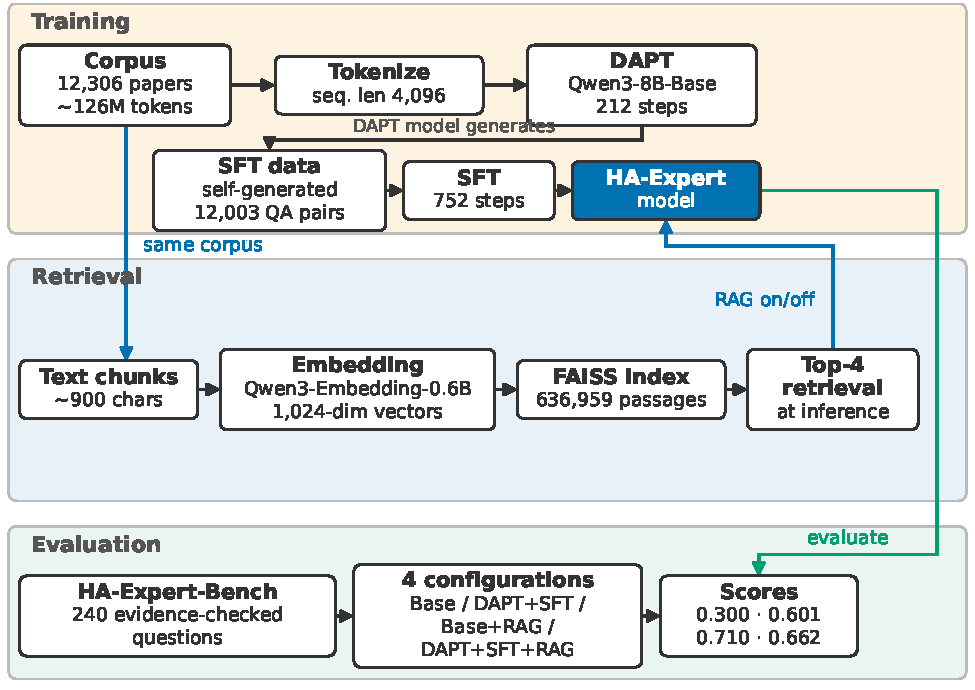
\includegraphics[width=\textwidth]{figs/fig1-pipeline.pdf}
\caption{The HA-Expert pipeline. \textbf{Training:} the 12,306-paper
corpus is tokenized for domain-adaptive continued pretraining (DAPT) of
Qwen3-8B-Base; the DAPT model then generates its own supervised
fine-tuning (SFT) data, grounding-filtered, for full-parameter SFT.
\textbf{Retrieval:} the same corpus is chunked and embedded into a FAISS
index of 636,959 passages; at inference the top-4 passages are prepended
to the question (RAG on) or the model answers from parameters alone
(RAG off). \textbf{Evaluation:} all four configurations --- base,
DAPT+SFT, and each with retrieval --- are scored on HA-Expert-Bench's
240 evidence-checked questions.}
\label{fig:pipeline}
\end{figure}

\subsection{Domain-adaptive pretraining (DAPT)}
\label{sec:dapt}

Starting from Qwen3-8B-Base~\cite{qwen3}, we ran full-parameter continued
pretraining on the DAPT sets of Section~\ref{sec:corpus}. Documents were
chunked at document boundaries to 4,096-token sequences
(legacy block packing) with SDPA attention. The effective
batch was 8 sequences $\times$ gradient accumulation 16, i.e.\ 128
sequences or 524,288 tokens per step. The learning rate was
$1\times10^{-5}$ with cosine decay. Training ran for 212 steps
($\approx$111M tokens) in 5\,h 34\,min on a single
RTX PRO 6000 (96\,GB), reaching a final training loss of $\approx$1.55.

On a 63-question development split, the DAPT model tied the base model on
the auto-graded items (5/6), even as it repaired knowledge traps the base
model missed: DAPT changed what the model \emph{knows} without changing
how it \emph{behaves}. That division of labor --- DAPT for
knowledge, a second stage for behavior --- motivated the SFT stage; the
full-bench results (Section~\ref{sec:experiments}) bear it out.

\subsection{Self-generated SFT data}
\label{sec:sft-data}

The DAPT model served as its own teacher, under this protocol:
\begin{enumerate}
\item Serve the DAPT model locally with vLLM~\cite{vllm} (zero API cost).
\item Sample passages from the corpus, excluding the 30 holdout papers of
Section~\ref{sec:corpus}.
\item Generate a question--answer pair conditioned on each passage,
anchoring every candidate answer to a specific source text.
\item Retain a pair only if the answer is \emph{grounded} in its source
passage, operationalized as a content-word overlap of $\geq 0.55$ between
the answer and the passage; deduplicate.
\end{enumerate}
Two generation rounds produced 5,403 and 6,600 retained pairs,
respectively, for \textbf{12,003 examples}. The filter checks
topical attestation, not truth (Section~\ref{sec:limitations}); the
benchmark's keys, by contrast, were verified by a separate
evidence-restricted process (Section~\ref{sec:bench}).

\subsection{Supervised fine-tuning}
\label{sec:sft-train}

SFT was full-parameter, in prompt/completion format with loss computed on
the completion only, at learning rate $1\times10^{-5}$ for 2 epochs
(752 steps), with NEFTune noise~\cite{neftune} 5.0 and an 8-bit Adam
optimizer. Training finished at train loss 1.214 in $\approx$19 minutes.
The base model's
signature pathology --- inventing follow-up questions instead of
answering --- disappeared from the fine-tuned model's outputs.

\subsection{Retrieval-augmented inference (RAG)}
\label{sec:rag}

For the retrieval mode, all 12,306 papers were chunked by merging
paragraphs to $\approx$900 characters, with a 150-character overlap on
long paragraphs, and embedded with Qwen3-Embedding-0.6B
(1,024-dimensional), giving a FAISS IndexFlatIP~\cite{faiss} index of
\textbf{636,959 passages}. Holdout papers are absent from the index. At
inference, the top-4 passages for a question are prepended to it with
citation markers [1]--[4], and the model is instructed to cite them in
its answer.

One decoding detail matters for interpreting the results: the public demo
decodes with a repetition penalty of 1.05, which largely suppresses the
repetition failure mode (Section~\ref{sec:analysis}), while the
benchmark evaluation (Section~\ref{sec:experiments}) deliberately uses
plain greedy decoding, so decoding aids do not mask the behavior
measured.

\section{HA-Expert-Bench}
\label{sec:bench}

\subsection{Composition}

HA-Expert-Bench contains 240 questions spanning seven content categories:
basics; history and industry; synthesis and chemistry; modification and
derivatives; molecular-weight biology and receptors; nano-delivery; and
experimental and clinical topics. Questions take four formats
(Table~\ref{tab:benchcomp}). \emph{Trap} questions embed a false premise
an expert should reject rather than answer on its own
terms --- e.g., ``HA solutions are simple Newtonian fluids, so their
viscosity is a single constant, correct?'' The trap format exists because
premise rejection was one of the three failure modes of
Section~\ref{sec:intro}, invisible to benchmarks that only ask
well-formed questions.

\begin{table}[t]
\centering
\begin{tabular}{lcll}
\toprule
Format & $n$ & Grading & Notes \\
\midrule
Open & 195 & LLM judge & free-form answers \\
Quantitative & 20 & automatic & numeric tolerance \\
Trap & 15 & LLM judge & false premise to reject \\
Multiple-choice & 10 & automatic & exact option letter \\
\midrule
Total & 240 & & \\
\bottomrule
\end{tabular}
\caption{HA-Expert-Bench composition. Judge-graded items use the
correct / partial / wrong rubric of Section~\ref{sec:grading}, scored
1.0 / 0.5 / 0.0 against the evidence-checked reference key.}
\label{tab:benchcomp}
\end{table}

\subsection{Evidence-checked answer keys}
\label{sec:keys}

Draft keys were not trusted as written. Each key passed through an
evidence-restricted verification protocol in which LLM verifiers received
an evidence pack of source passages and could take exactly three actions:
\emph{confirm} the key, \emph{correct} it while quoting the decisive
passage, or mark it \emph{uncertain} --- never asserting facts from
outside the pack.

\textbf{Round one (keyword evidence).} Evidence packs were assembled by
tracing each question to its source paper (38 questions) or by keyword
retrieval over the corpus (202 questions). Outcome: 118 keys verified,
19 corrected, 103 marked uncertain.

\textbf{Round two (vector evidence).} The 103 uncertain keys were
re-verified against evidence packs of the top-6 passages retrieved from
the vector index of Section~\ref{sec:rag}, under the same three-action
protocol. Outcome:
72 verified, 3 corrected, 28 still uncertain.

\textbf{Released key set (v3).} Across both rounds, 190 keys are verified
and 22 corrected, so \textbf{212 of 240 keys (88.3\%) are
evidence-settled}; the remaining 28 (11.7\%) are released flagged as
uncertain drafts. Only three keys changed in round two (B22 and F07,
quantitative; G14, trap). Since scores had been computed against the v2
keys, we re-scored these three under v3: B22 and F07 auto-grades are
identical in all four cells, and G14's verdicts are unchanged on
re-judging, so all scores in Section~\ref{sec:experiments} stand under
the released v3 keys. Every per-question verification status is
published with the benchmark.

\subsection{Grading protocol}
\label{sec:grading}

Multiple-choice items are graded by exact option letter and quantitative
items by numeric tolerance; both are fully automatic. Open and trap items
are graded by an LLM judge shown the question, the evidence-checked
reference answer, and the model's response, and required to return a
verdict of correct, partial, or wrong, scored 1.0, 0.5, and 0.0
respectively. The judge was the SFT model itself, served locally --- a
deliberate \$0 choice whose bias implications we treat as a limitation
(Section~\ref{sec:limitations}). Two features of the protocol mitigate,
without eliminating, that bias: anchoring to a fixed verified
reference key rather than a free pairwise preference, and the 30
automatic items as a judge-free control
(Section~\ref{sec:experiments}). Judge outputs that failed to parse were
re-judged in a retry pass, which moved overall scores by at most 0.004;
the residual ungraded items are accounted for in
Section~\ref{sec:experiments}.

\section{Experiments and Results}
\label{sec:experiments}

\subsection{Protocol}

We evaluate four cells under a single protocol: the base model
(Qwen3-8B-Base); the adapted model (DAPT+SFT); and each with
retrieval (base+RAG, DAPT+SFT+RAG). Responses for all 240 questions were
generated with greedy decoding (temperature 0, maximum 512 tokens) on a
single RTX PRO 6000 (96\,GB), graded as in
Section~\ref{sec:grading}. Some items remained ungraded because the judge's output was
unparseable even after the retry pass (judge JSON failures): 13 (base),
23 (DAPT+SFT), 2 (base+RAG), and 21 (DAPT+SFT+RAG),
leaving $n = 227$, $217$, $238$, and $219$ graded responses per cell.
Following the judge's known limits, we treat cross-cell gaps
below $\approx$0.02 as noise.

\begin{table}[t]
\centering
\begin{tabular}{lccccc}
\toprule
Cell & Overall & MCQ (10) & Quant.\ (20) & Open (195) & Trap (15) \\
\midrule
Qwen3-8B-Base        & 0.300 & 0.800 & 0.250 & 0.282 & 0.267 \\
+ DAPT \& SFT        & 0.601 & \textbf{0.900} & 0.300 & 0.631 & 0.500 \\
+ RAG                & \textbf{0.710} & \textbf{0.900} & 0.450 & \textbf{0.719} & \textbf{0.867} \\
+ DAPT \& SFT \& RAG & 0.662 & 0.700 & \textbf{0.550} & 0.676 & 0.633 \\
\bottomrule
\end{tabular}
\caption{HA-Expert-Bench results (240 questions; means over graded items,
$n$ per cell as in Section~\ref{sec:experiments}). Bold marks the best
score in each column. Three facts organize the table: fine-tuning doubles
the base model; retrieval on the \emph{base} model beats the full
training pipeline without it; and the combination underperforms
retrieval alone on open and trap questions while posting the best
quantitative score. On the 30 auto-graded items alone (no judge):
0.433 / 0.500 / 0.600 / 0.600, same cell order.}
\label{tab:main}
\end{table}

\begin{figure}[t]
\centering
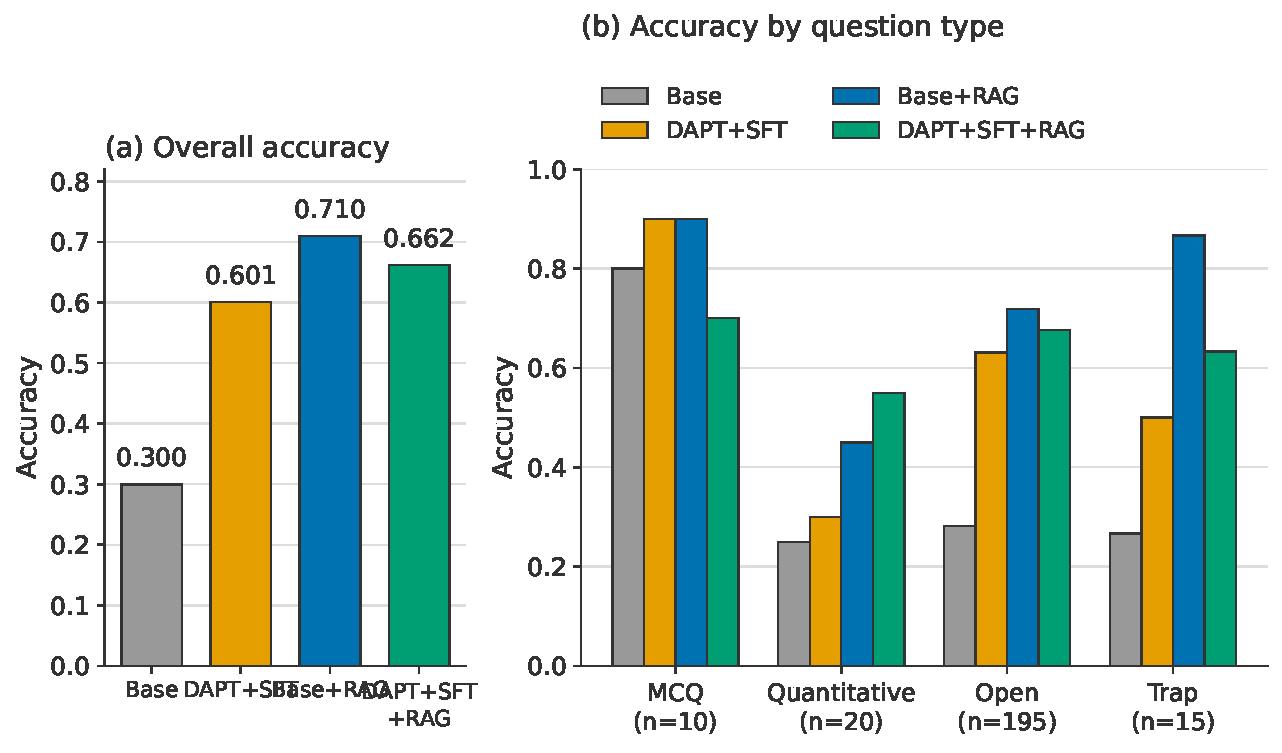
\includegraphics[width=\textwidth]{figs/fig2-results.pdf}
\caption{HA-Expert-Bench results by configuration (240 questions;
per-cell graded $n$ as in
Section~\ref{sec:experiments}). (a) Overall accuracy: fine-tuning
doubles the base model (0.300 $\rightarrow$ 0.601), retrieval alone is
worth more (0.710), and the two do not compose additively (0.662).
(b) By question type: retrieval's largest effect is on traps
(0.267 $\rightarrow$ 0.867 for the base model); the
combined cell posts the best quantitative score (0.550). Colors match
Figure~\ref{fig:failures}.}
\label{fig:results}
\end{figure}

\subsection{Fine-tuning doubles the base model}

DAPT+SFT scores 0.601 overall against the base model's 0.300
(Table~\ref{tab:main}, Figure~\ref{fig:results}). The gain is
largest where the base model's deficit was behavioral: open
questions rise from 0.282 to 0.631, because the fine-tuned model answers
the question asked rather than continuing the prompt --- confirming the
division of labor from the development check (Section~\ref{sec:dapt}).
Trap accuracy also improves
(0.267 $\rightarrow$ 0.500) but remains unreliable.

\subsection{Retrieval is the largest single lever}

Adding retrieval to the \emph{base} model
scores 0.710, beating the full pipeline without it
(0.601). The effect is largest where parametric knowledge is
least reliable: trap accuracy rises from 0.267 to 0.867. Both parametric
trap failures (G01, ``HA is a protein polymer'';
G13, ``HA solutions are Newtonian fluids'') are corrected by both
retrieval cells. The pattern has a simple reading: a false premise is
hard to reject from memory, but easy when the contradicting passage is
in the prompt. Retrieval converts an epistemic problem into a reading
problem, and reading is what base models already do well.

\subsection{SFT and RAG interfere}

The combined cell, DAPT+SFT+RAG (0.662), trails base+RAG overall despite
dominating it without retrieval. The deficit is concentrated in the two
judge-graded formats: open (0.676 vs.\ 0.719) and trap (0.633
vs.\ 0.867). It is not uniform: on quantitative questions the combined
cell posts the best score of any cell (0.550, vs.\ 0.450 for base+RAG),
as if trained domain numeracy composes with retrieved figures when the
answer is a number, while the interference appears where the model must
produce grounded prose. A judge-free control supports localizing the
effect this way: on the 30 auto-graded items, DAPT+SFT+RAG \emph{ties}
base+RAG (0.600 each), so the headline gap lives in the judged formats,
not in the objective subset. Section~\ref{sec:analysis} identifies the
mechanism.

\section{Analysis}
\label{sec:analysis}

\subsection{Mechanism 1: a train/test format mismatch}

The SFT data (Section~\ref{sec:sft-data}) consists exclusively of bare
question$\rightarrow$answer pairs, so the fine-tuned model never saw the
RAG cells' input format in training: a question preceded
by four retrieved passages and an instruction to cite them. On 5 of 240
such inputs, the model collapses into a \emph{citation-marker loop} ---
citation markers repeated to the token limit
(``[1] [4] [2] [3] [1] [4] [2] [3] $\ldots$'') --- scoring zero on
questions the same model answers correctly without retrieval. The
failure is diagnostic rather than random: the citation markers are the
most salient novel tokens in the unseen format, and a model trained to
continue its prompt's pattern continues them. This is an account
of a \emph{training-data omission}, not of retrieval hurting a
well-matched model; Section~\ref{sec:future} describes the fix.

\subsection{Mechanism 2: repetition inherited through self-distillation}

We define \emph{heavy repetition} operationally as a 30-character block
repeated at least $5\times$ within one response. It appears in 35 of 240
DAPT+SFT responses, against 10 of 240 for the base model, with retrieval
lowering both cells (7 and 22 of 240; Figure~\ref{fig:failures}). Because the
SFT teacher \emph{was} the DAPT model (Section~\ref{sec:sft-data}), the
natural reading is that its repetition habit was distilled into the
student: self-distillation transmits behavior,
including degenerate behavior, and a content-word grounding filter does
not screen for it. Repetition is also the more tractable failure mode
--- it is decode-sensitive, and largely suppressed in the demo
(Section~\ref{sec:rag}) --- but under the
benchmark's unaided greedy decoding it is part of what is measured.

\begin{figure}[t]
\centering
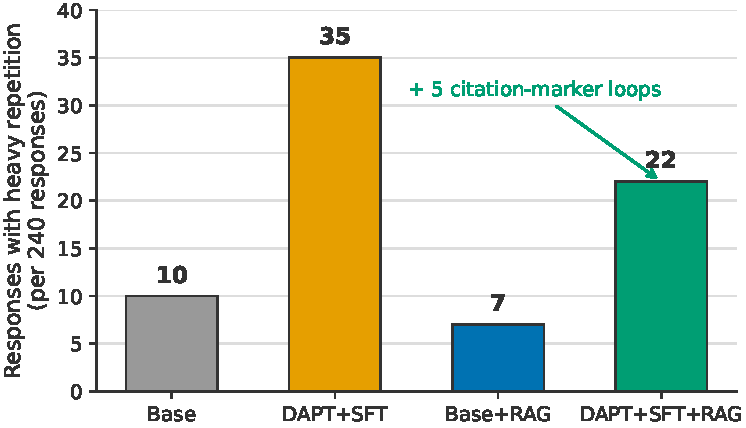
\includegraphics[width=0.85\textwidth]{figs/fig3-failure-modes.pdf}
\caption{Failure-mode counts per configuration (240 responses each,
greedy decoding). \emph{Heavy repetition} is a 30-character block
repeated at least $5\times$ within one response. Fine-tuning on
self-generated data more than triples the base model's count
(10 $\rightarrow$ 35), consistent with the teacher's repetition habit
being distilled into the student; retrieval lowers both
counts. The annotation marks Mechanism 1's 5 citation-marker loops,
only in the DAPT+SFT+RAG cell.}
\label{fig:failures}
\end{figure}

\subsection{Case studies}

The two mechanisms are visible in their purest form on trap items, where
the correct behavior --- rejecting the premise --- is unambiguous.

\textbf{G13 --- ``HA solutions are simple Newtonian fluids, so their
viscosity is a single constant, correct?''} The SFT model assents, then
repeats itself: \emph{``Yes, HA solutions are simple Newtonian
fluids, so their viscosity is a single constant.''} The same model with
retrieval corrects the premise precisely: \emph{``No, HA solutions are
not simple Newtonian fluids. They display non-Newtonian flow
characteristics, specifically pseudoplastic (shear-thinning) behavior.
This means that their viscosity decreases as shear rate increases.''}

\textbf{G09 --- ``For joint injections, the highest-MW HA is always the
best choice, correct?''} The SFT model correctly rejects the absolute:
\emph{``No, the highest-MW HA is not always the best choice for joint
injections. The choice of HA depends on the specific condition being
treated\ldots''} The SFT+RAG response degenerates
entirely into a citation-marker loop (``[1] [4] [2] [3] [1] [4] [2] [3]
$\ldots$'', to the token limit). Retrieval, which rescues G13, destroys
G09 --- the interference of Section~\ref{sec:experiments} in
a single response, on a question the parametric model gets right.

\begin{table}[t]
\centering
\begin{tabular}{lcccc}
\toprule
Trap & Base & SFT & Base+RAG & SFT+RAG \\
\midrule
G01 & wrong   & wrong   & correct & correct \\
G02 & wrong   & wrong   & correct & wrong \\
G03 & wrong   & wrong   & correct & partial \\
G04 & partial & correct & correct & correct \\
G05 & partial & correct & correct & correct \\
G06 & partial & correct & correct & wrong \\
G07 & partial & correct & partial & partial \\
G08 & partial & correct & correct & correct \\
G09 & wrong   & correct & partial & wrong \\
G10 & wrong   & ungraded & partial & partial \\
G11 & wrong   & wrong   & correct & correct \\
G12 & correct & ungraded & correct & wrong \\
G13 & wrong   & wrong   & correct & correct \\
G14 & wrong   & wrong   & correct & correct \\
G15 & partial & partial & partial & correct \\
\bottomrule
\end{tabular}
\caption{Per-question verdicts on the 15 trap items. Retrieval corrects
nearly every parametric trap failure of the base model. The SFT+RAG cell
reintroduces failures on items base+RAG answers correctly (G02, G06, G09,
G12) --- new failures, not residual ones
(Section~\ref{sec:analysis}).}
\label{tab:traps}
\end{table}

\section{Limitations}
\label{sec:limitations}

\textbf{The judge is one of the contestants.} Open and trap items are
graded by the SFT model itself (Section~\ref{sec:grading}). Anchoring to
a fixed, evidence-checked reference key --- rather than free pairwise
preference --- and the judge-free auto-graded control (on which the
combined cell ties base+RAG) bound the plausible distortion, but do not
eliminate it. An external judge is the obvious upgrade.

\textbf{Residual key uncertainty.} 28 of 240 keys (11.7\%) remain
uncertain drafts, and scores on those items carry key risk. Verification
also \emph{changed} 22 of 240 keys (9\%) across two rounds: a benchmark
built from unchecked model-written keys would have carried that error
rate silently into every score --- including, here, the scores of the
very model that wrote the drafts.

\textbf{Small cells.} The multiple-choice column rests on $n=10$: the
SFT+RAG dip there (0.700 vs.\ 0.900) is exactly two questions, and we draw
no conclusion from it. Trap ($n=15$) verdicts are similarly coarse, and
are reported per question (Table~\ref{tab:traps}) rather than
only as a mean.

\textbf{The grounding filter checks attestation, not truth.} A
content-word overlap of $\geq 0.55$ establishes that an answer is about a
real passage, not that it states the passage correctly, so self-generated
SFT data can encode teacher errors despite the filter of
Section~\ref{sec:sft-data}. The repetition inheritance of
Section~\ref{sec:analysis} is one measured consequence; factual
contamination of the same kind cannot be excluded and would require
expert audit of the training set.

\textbf{Decoding and seed.} All results use a single greedy-decoding run.
Repetition behavior is decode-sensitive, so Mechanism 2's absolute
size is a property of model-plus-decoding, not of the model alone.

\textbf{Scale and scope.} One 8B model in one narrow domain: the
transferable claim is the pipeline and its failure analysis, not any
absolute score, and the interference result should be re-checked at other
scales and domains before being treated as general.

\textbf{Replicability.} Nothing in the pipeline is HA-specific beyond the
corpus query: harvest $\rightarrow$ clean $\rightarrow$ DAPT $\rightarrow$
self-generated grounded SFT $\rightarrow$ evidence-checked bench
$\rightarrow$ four-cell ablation, at a total cloud compute cost of under
USD 50. For small
fields with open-access literatures, this is a realistic template for a
first trustworthy domain model --- and the interference result is a
warning worth having before, not after, combining SFT with retrieval.

\section{Future Work}
\label{sec:future}

Section~\ref{sec:analysis} points to one fix per mechanism. For the
format mismatch: \emph{retrieval-formatted SFT data} --- training
examples in the exact inference format (question + retrieved excerpts +
cited answer), so the model learns to use context instead of
collapsing on it; we predict this alone should move the combined cell
above base+RAG, a prediction directly testable with the released
pipeline. For the repetition inheritance: \emph{repetition filtering}
of teacher outputs before SFT, screening generated pairs with the
operational definition used to measure the failure, so the habit is never
distilled; repetition-aware decoding remains an inference-side
mitigation. On the evaluation side, re-grading with an external judge
and settling the 28 remaining uncertain keys would tighten every
comparison in Table~\ref{tab:main}.

\section{Data and Code Availability}
\label{sec:availability}

\begin{itemize}
\item Code, corpus manifests, benchmark (v3 keys with per-question
verification status), and full result files:
\url{https://github.com/liukunli001/hyaluronan-expert-llm}
\item Weights: \url{https://huggingface.co/liukunli/ha-expert-qwen3-8b}
(SFT model) and
\url{https://huggingface.co/liukunli/ha-expert-qwen3-8b-dapt} (DAPT
checkpoint)
\item Retrieval index:
\url{https://huggingface.co/datasets/liukunli/ha-expert-index}
\item Interactive demo (chat + cited retrieval):
\url{https://huggingface.co/spaces/liukunli/ha-expert-demo}
\item Corpus release: GitHub Release \texttt{v0.1-data}.
\end{itemize}

\section*{Acknowledgements}

This is an independent research project; the author thanks the open-access
publishers whose PMC deposits made the corpus possible, and the Qwen,
Hugging Face, vLLM, and FAISS communities for the tooling.

\begin{thebibliography}{9}

\bibitem{qwen3}
Qwen Team.
\newblock \emph{Qwen3 Technical Report}.
\newblock Alibaba Group, 2025.

\bibitem{transformers}
Wolf, T., et al.
\newblock Transformers: State-of-the-Art Natural Language Processing.
\newblock In \emph{Proceedings of EMNLP 2020: System Demonstrations}.

\bibitem{trl}
von Werra, L., et al.
\newblock \emph{TRL: Transformer Reinforcement Learning}.
\newblock Hugging Face library, 2023.

\bibitem{neftune}
Jain, N., et al.
\newblock NEFTune: Noisy Embeddings Improve Instruction Finetuning.
\newblock \emph{arXiv:2310.05914}, 2023.

\bibitem{fineweb}
Penedo, G., et al.
\newblock The FineWeb Datasets: Decanting the Web for the Finest Text Data
at Scale.
\newblock In \emph{Advances in Neural Information Processing Systems
(NeurIPS)}, 2024.
\newblock (FineWeb-Edu subset used for replay.)

\bibitem{vllm}
Kwon, W., et al.
\newblock Efficient Memory Management for Large Language Model Serving
with PagedAttention.
\newblock In \emph{Proceedings of SOSP}, 2023.

\bibitem{faiss}
Johnson, J., Douze, M., and J\'egou, H.
\newblock Billion-Scale Similarity Search with GPUs.
\newblock \emph{IEEE Transactions on Big Data}, 7(3):535--547, 2021.

\end{thebibliography}

\end{document}
